\chapter{\label{chap:testprep}System Test Preparation}

The GMAT system tests are designed to perform a ``black box'' examination of GMAT as an assembled
system.  The system tests exercise all of the elements of the system from both the scripting and
graphical user interface perspectives.  Traceability matrices are maintained to ensure that the
entire system is exercised upon completion of the system tests.  This chapter describes these
matrices, and provides instructions about how to maintain and extend them.

\section{Test Process}

\begin{figure}[htb]
\begin{center}
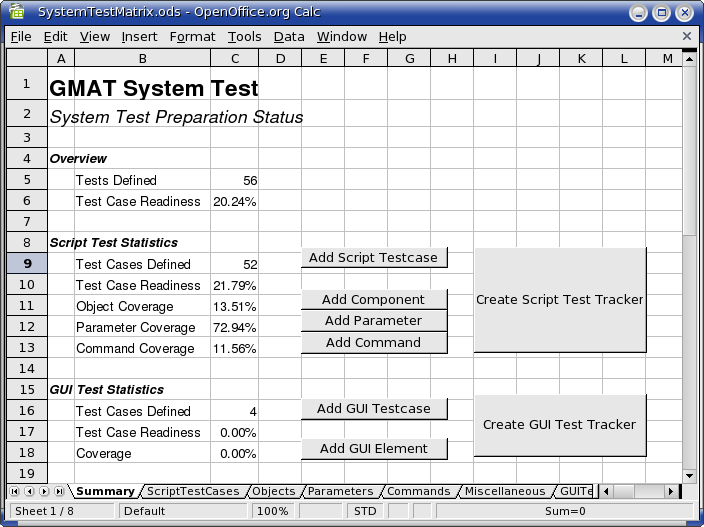
\includegraphics[400,300]{Images/SystemTestSummary.png}
\caption{\label{figure:SystemTestSummary}The System Test Summary Page}
\end{center}
\end{figure}

System testing is performed in three stages: test preparation, system testing (consisting of Script
based Testing and GUI Testing), and test result reporting.  The test preparation
phase, described in this chapter, is used to update the system test cases with tests covering new
capabilities of GMAT, and to add or update existing test cases based on lessons learned from
previous testing.  Procedures followed when executing the script based are described in
Chapter~\ref{chap:scripttests}.  GUI testing procedures are given in Chapter~\ref{chap:guitests}.
Both of those chapters include descriptions of the data collection for individual tests.
Chapter~\ref{chap:reporting} describes the process of accumulating the test results so that the
status of the system can be evaluated.

\section{Test Preparation}

GMAT system testing is managed from a set of OpenOffice\cite{OOo} spreadsheets.  The test case
structure and mapping between system functionality and corresponding tests is tracked using the
"SystemTestMatrix.ods" spreadsheet\footnote{All of the GMAT test tracking components are
configuration controlled.  Interested parties can obtain the current versions of these testing
artifacts by contacting one of the GMAT team leads.}. This spreadsheet contains pages identifying
detailed GMAT functionality and defined system test cases, and maps each element of functionality to
one or more test cases.

The spreadsheet includes a summary page, shown in Figure~\ref{figure:SystemTestSummary}, which
computes coverage for the elements tabulated on the detail pages.  If the tables in the spreadsheet
are up to date, then the summary page is an indicator of the readiness of the system tests.  Hence
the first task that testers perform when preparing for system testing is to update the test
matrices.  Once the test matrices have been updated, the test cases are updated to cover any new
functionality in the system.  Test preparation is finished when a complete set of test cases has
been developed, covering all of the elements in the updated test matrix tables.

\begin{figure}[htb]
\begin{center}
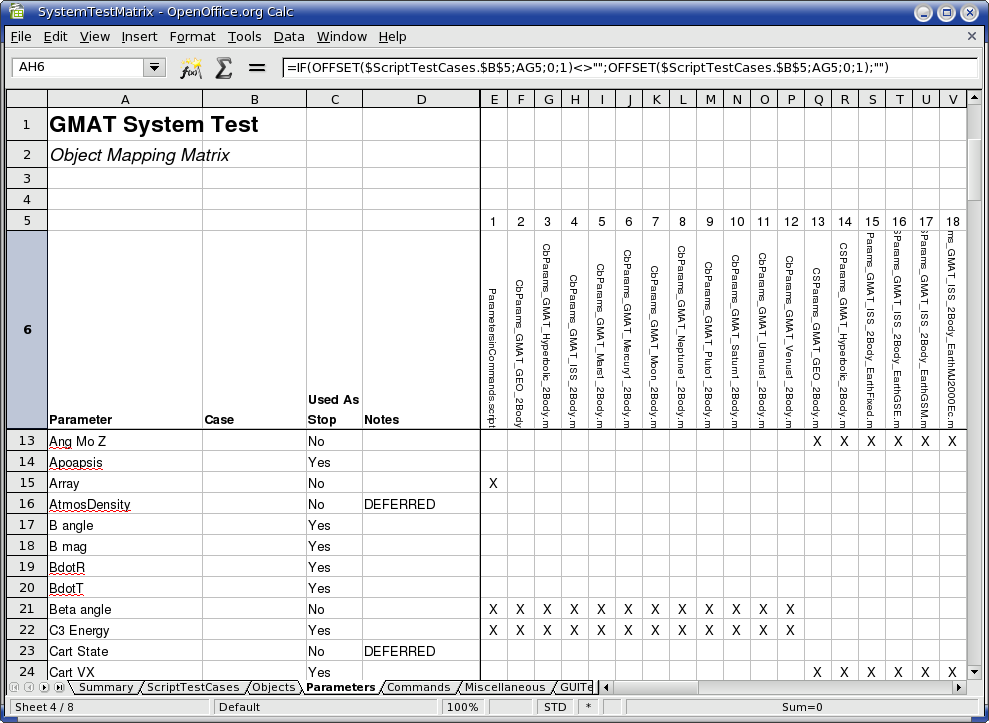
\includegraphics[400,300]{Images/ComponentTestMatrix.png}
\caption{\label{figure:ComponentTestMatrix}An Object Test Matrix}
\end{center}
\end{figure}

To summarize, when a new piece of functionality is added to GMAT that users can access, the test
team, working with the developers and users, updates the test matrices by performing three steps:

\begin{enumerate}
\item Identify and add all new elements of the system to the test matrices.
\item\label{item:planTheWork} Identify test cases that cover the new elements.  This may involve
modifying existing test cases or creating new test cases, depending on the functionality of the new
element.
\item Create or update the test cases as needed to implement the planned coverage identified in
item~\ref{item:planTheWork}.
\end{enumerate}

When these steps have been performed, the coverage matrices are up to date, and the test team is
ready to run the system test by executing all of the test cases in the matrices.  The following
paragraphs describe the procedure for executing these steps.


\section{Updating the Element Lists in the Test Matrices}

Figure~\ref{figure:ComponentTestMatrix} shows an example of the matrices used to identify GMAT's
implemented functionality.  Separate tables exist for the user accessible Components (Spacecraft,
Solvers, Propagators, and so forth), Parameters that GMAT can calculate, Commands used when defining
the mission sequence, Graphical User Interface elements (GuiElements), and miscellaneous other
configurable elements.  These tables capture a static view of every item that a user can interact
with when running GMAT.

Each table lists the configurable elements in column A, and constructs, when appropriate,
configurations and subconfigurations of those objects in columns B~(labeled ``Cases'') and
C~(``Subcases'').  Column D, ``Notes'', is used to indicate other considerations.  Elements that are
not yet scheduled for testing can be entered in the tables; when that happens, the entry in the
``Notes'' column should be set to the keyword ``DEFERRED''.

The first step in updating the test matrices is to ensure that the lists of accessible elements are
complete, capturing any new elements and configurations added to the system since the last time the
matrix was updated.  Testers have two options for performing these updates: they can either edit the
tables by hand, and check that all related formatting and equations are updated correctly, or they
can use the macros built into the spreadsheet to add the new elements.  The preferred approach is to
use the macros, because that approach ensures that the calculations performed by the tables are
correct.

\begin{figure}[htb]
\begin{center}
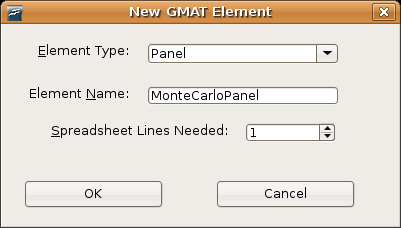
\includegraphics[200,114]{Images/AddingAnElement.png}
\caption{\label{figure:NewElement}The New Element Dialog}
\end{center}
\end{figure}

The summary page, shown in Figure~\ref{figure:ComponentTestMatrix}, for the spreadsheet contains
four buttons used to add elements to the test matrices: ``Add Resource'', ``Add Parameter'', ``Add
Command'', and ``Add GUI Element''.  When a user presses one of these buttons, a dialog box opens
that is used to set some basic information for the new element that is being tested.
Figure~\ref{figure:NewElement} shows an example of this dialog.

When this dialog is opened, users can change the type of new element being configured using the
Element Type combo box.  This option is provided in case the user selected the wrong button from the
summary page.  The user enters the name of the new element in the ElementName field.

Many of the elements that are tested can be exercised more than one way; for example, the Impulsive
Burn element can be set to run using Velocity-Normal-Binormal (VNB) delta-V vectors or a coordinate
system based delta-V vector.  Each of these modes should be tested independently, so a separate line
should exist for each on the spreadsheet.  The user reserves multiple lines on the spreadsheet by
entering the number of lines required in the ``Spreadsheet Lines Needed'' field.

After setting the data correctly on the new element dialog, the user presses the `OK'' button.  When
this action is taken, the test matrix corresponding to the type of the new element is updated. New
rows are inserted into the spreadsheet for the new element, and the formulas for the new rows are
set.  Finally, the fields that are used to calculate the test preparation statistics are updated.
If more than one row was inserted, the spreadsheet page is set to the page containing the new
element, with the active cell selected to the ``Cases'' field for the new element, so that the user
can enter the test cases required for the new element.  Each test case and subcase should be entered
at this time so that the element descriptions in the test matrix reflect the capabilities that need
to be tested.

At this point, all of the functionality in GMAT should be represented by rows in the test matrices.
The next step is to plan test cases that cover elements of the system that are not already handled
in the test suite.

\begin{figure}[h!]
\begin{center}
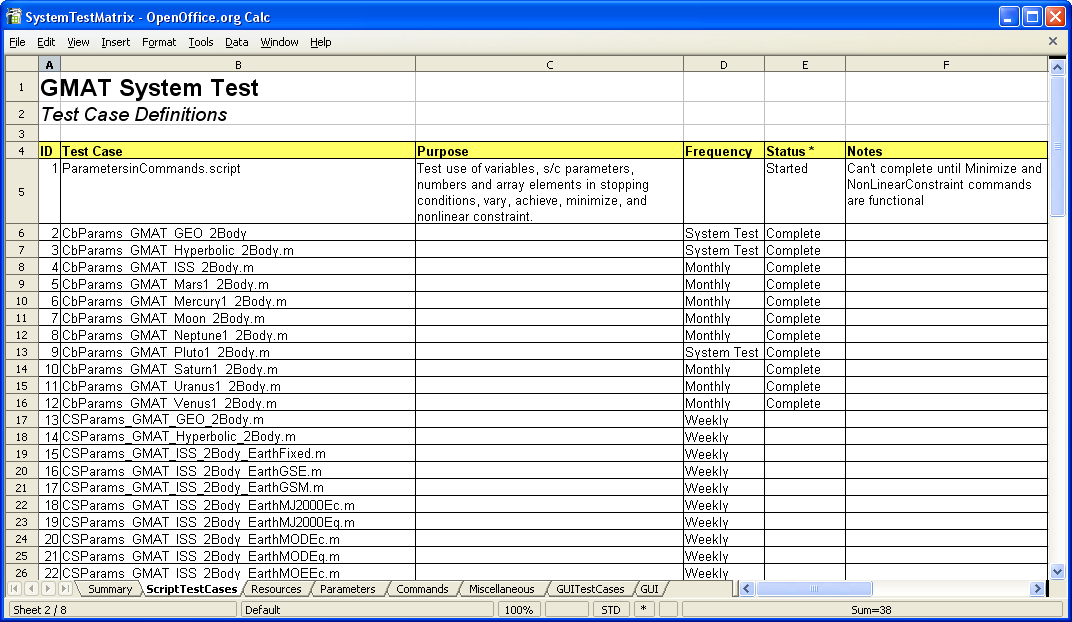
\includegraphics[460,289]{Images/TestCaseTable.png}
\caption{\label{figure:TestCaseTable}A Test Case List}
\end{center}
\end{figure}

\section{Updating the Test Case Lists}

There are two categories of test cases used in system testing GMAT, designed to exercise the system
using scripting and the graphical user interface.  When new components are added to GMAT, the test
coverage matrix is updated to exercise those new elements using the procedure described above.  This
update produces holes in the system test suite, requiring either an update of the current test cases
or the development of new test cases, depending on the nature of the new components.

The test case lists are broken into two groups: tests based on script files designed to exercise all
components used in modeling a mission, and user interface exercises designed to test the
functionality and completeness of the graphical user interface.  The test tracking spreadsheet has
separate pages for the GUI and script based test cases.  Figure~\ref{figure:TestCaseTable} shows the
page for the script cases; the GUI test case page is similar.

When a test case is added to the test case list using the spreadsheet macros described below, that
test case name is automatically picked up on the coverage tables.  Once this update has been made
and the new test cases have been added to the system test suite, users of the test matrix
spreadsheet edit the matrices to indicate the covered functionality.  In summary, the procedure for
incorporating a new test case is to perform these three steps:

\begin{enumerate}
\item \emph{Test case planning:} Identify and name the new test cases, and update the spreadsheet to
list these cases.
\item \emph{Test case writing:}  Write the new test cases, and update any older test cases that need
updating.
\item \emph{Test Matrix Mapping:}  Working from the new test cases, fill in the coverage tables for
each new or changed test case to reflect the features actually covered.
\end{enumerate}

\begin{figure}[h!]
\begin{center}
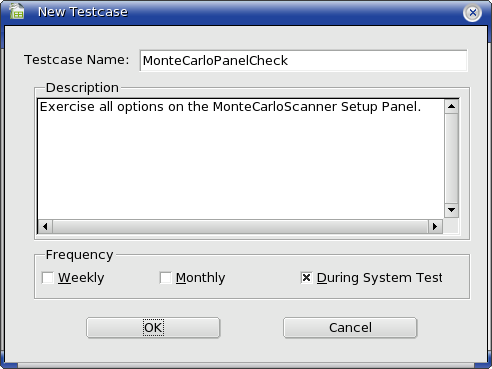
\includegraphics[246,185]{Images/AddingAGuiCase.png}
\caption{\label{figure:AddATestCase}The New Test Case Dialog}
\end{center}
\end{figure}

The procedure for adding a test case to the test case list is similar to the procedure for adding a
new element to the test matrices.  Test cases are added to the system test matrices using the ``Add
Script Testcase'' and ``Add GUI Testcase'' buttons on the summary page of the spreadsheet.  Pressing
either of these buttons opens the New Test Case dialog, shown in Figure~\ref{figure:AddATestCase}.

When a new test case has been identified, a user will open the system test spreadsheet and press the
button for the desired test case type, opening this dialog.  The user then enters the name of the
new test case.  The user enters a summary description of the test case as well to help track the
goal of the test case.  Finally, the user selects the desired frequency for execution of the test
case; cases that can be automated and run frequently, or that test critical features of the system,
should be set to run more frequently than those that are labor intensive or that test rarely used
GMAT features.

The user accepts the new test case by selecting the ``OK'' button on the spreadsheet.  When this
action is taken, several things happen in the tables in the spreadsheet.  First new test case is
added to the appropriate page of the spreadsheet, along with its descriptions and execution
frequency.  The status of the test case is set to ``Not started'', indicating that the test case
itself is not yet in the system test suite of test cases.  The new test case is added to the column
labels of the test matrices on the subsequent pages, and the formulae in in the spreadsheet are
updated to track the new tests.

This step completes the test case planning phase of the preparation process.  The next step is to
write the test cases themselves.

\section{Constructing the Test Cases}

The steps described so far ensure that there is a plan in place to test every element of GMAT for a
black box perspective.  At this point, the test cases requires for the system test have been
identified.  Next the test team needs to write the test cases, given the new functionality of the
system.  The goal for each test case is to test an integrated set of system elements when executing
a specified set of goals.

For the script based tests, this usually involves assembling a set of elements together and
performing some computations in a mission sequence.  The results of the execution of the script are
compared to known good data in order to validate that the execution behaved as expected.
Additionally, the script based testing checks to see that scripting errors are handled gracefully,
producing error messages that are clear for typical GMAT users.

GUI based scripts have similar goals.  The goals of the GUI test cases are to ensure that the GMAT
user interface lets users configure all of the elements of the system, that this configuration is
reflected in the internal components of the system, and that the user interface handles anomalous
conditions robustly.

The following paragraphs describe the approach taken to ensure that these goals are met.

\subsection{Updating Script Based Test Cases}

Script based test cases consist of a script file and validated output files generated from the
script.  All script based tests should be created from the GMAT GUI, so that any related user
interface issues can be identified during the process.  Once a scripted test has been constructed,
it should be saved with the same file name as entered in the test case table.

Each script based test should generate output in the form of a text file, using GMAT's reporting
capabilities.  Unless explicitly stated otherwise, the output file name should be the same as the
script file name with the file extension ``.report''.  The header comments on the script based tests
should indicate the following information:

\begin{itemize}
\item The first line of the script should be ``\%\% \$Id\$''.  This ensures that the CVS
version information is stored with the script.  This CVS information is the tracking identifier for
each system test case.
\item The primary elements being tested.
\item Any ancillary items that should also be examined in the execution of the test.
\item Any dependencies that need to be met to run the test successfully.  For example, the
FminconOptimizer requires a GMAT build that includes the MATLAB interfaces, a valid licensed MATLAB
executable on the test machine, and a valid licensed copy of MATLAB's Optimization Toolbox.
\item The name of the output files generated, is their name differs from the standard output file
name.
\item Whether the output data is expected to match data from previous runs.
\item Any special steps that should be taken, either prior to the run or after it completes.
\end{itemize}

\noindent A sample script test case is provided here:

\begin{quote}
\VerbatimInput[numbers=left,firstnumber=1]{./SystemTests/BasicProp.m}
\end{quote}

If a script test case fails any of the system test criteria specified in
Chapter~\ref{chap:scripttests}, the tester creates a test report summarizing the nature of the
failure.  A sample completed report is shown here:

\begin{quote}
\VerbatimInput[numbers=left,firstnumber=1]{./SystemTests/MatlabApsidesCheck.txt}
\end{quote}

\subsection{Updating the GUI Test Cases}

GUI based test cases consist of a text file describing the test.  The GUI test cases may include
additional files, depending on the nature of the test.  For example, the script reading GUI test
includes a script that needs to be read.  The purpose of the GUI tests is to validate that the
build is stable, and that the user interface panels provide complete coverage of the elements of
the system visible to the user.

The GUI test cases forms are relatively simple.  They provide, in outline form, guidelines for
testing the GUI elements.  Detailed instructions for the GUI tests are provided in
Chapter~\ref{chap:guitests}.

A sample GUI test case is provided here:

\begin{quote}
\VerbatimInput[numbers=left,firstnumber=1]{./SystemTests/ImpulsiveBurnPanel.txt}
\end{quote}

Failed GUI tests provide information about the nature of the failure durectly on the test case
form; there is no supplementary report for GUI test failures.

\section{\label{section:CompleteCoverage}Ensuring Complete System Coverage}

Once the test cases have been written, all that remains for test proparation is the confirmation
that the test cases cover all of the new features of GMAT.  This is accomplished by updating the
test matrices based on the new and revised test cases.  Each test case that has been added or
changed since the last update is collected and used to update the matrices.  For each page in the
spreadsheet containing an element to test case table, the test team needs to update the matrix
for these test cases.  The test cases are listed across the top of the matrices.  Each test case
identifies the tested elements by placing an ``X'' marker in the row corresponding to that element.
 Updated test cases should be examined to ensure that elements previously tested are still tested;
if an elemnet is no longer tested for a specific test case, the X for that element should be
removed from the matrix.

The spreadsheet contains formulas that use these markers to determine if a given element has a
corresponding test case.  The far right side of the test matrices tables accumulates this data;
every element that has at least one associated test case receives a coverage value of 1; uncovered
elements receive a coverage value of 0.  The far right side of the table also includes a column
labeled ``Row Count.'' The row count column simply counts the number of elements on the page.

\begin{figure}[htb]
\begin{center}
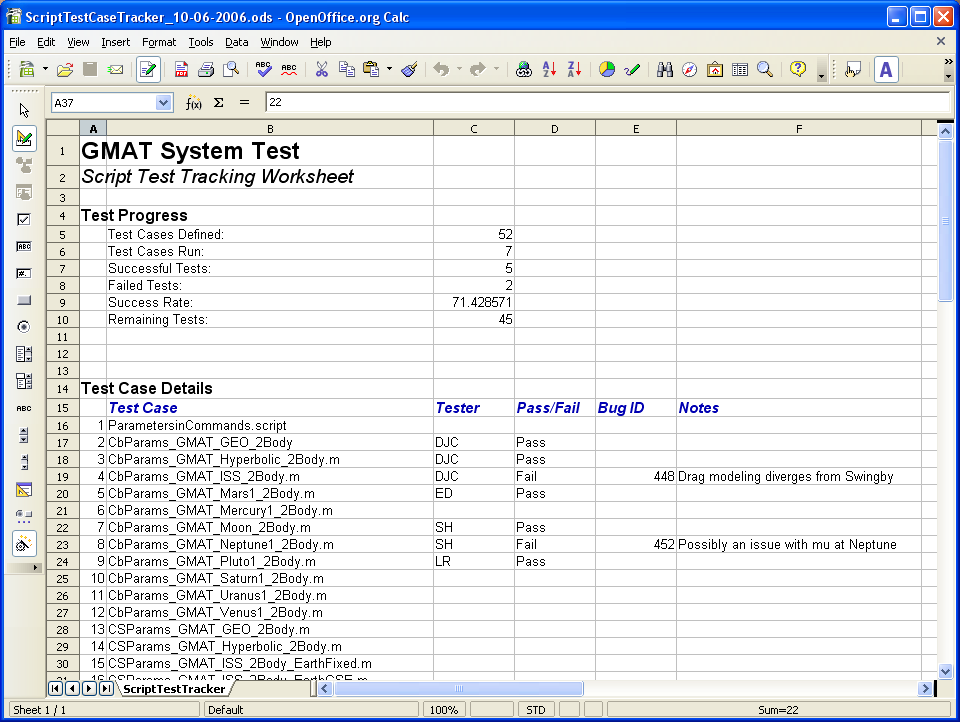
\includegraphics[460,346]{Images/TestTrackingWorksheet.png}
\caption{\label{figure:ScriptTestTracker}A Test Tracking Spreadsheet}
\end{center}
\end{figure}

The summary page examines each table in the spreadsheet and provides information about the
coverage completeness of the system tests.  Once the coverage statistics report that the elements
of the system are covered 100\%, the system tests are ready to be run.  The test team then
generates a new spreadsheet for each type of system test by pressing the ``Create Script Test
Tracker'' and ``Create GUI Test tracker'' buttons on the summary page.  These buttons generate
single page spreadsheets used to track progress through the system test.  An example is shown in
Figure~\ref{figure:ScriptTestTracker}.

This spreadsheet is used to track and report system test progress.  As each system test is
performed, the entry in the tracking spreadsheet is updated by the test team.  Examination of this
spreadsheet provides a status check on the system test.

The next two chapters provide instructions about the steps performed when running the system tests.
